\documentclass[10pt]{report}
\usepackage{/Users/bradenhoagland/latex/math}

\lhead{Braden Hoagland}
\chead{Topology}
\rhead{}

% make all mathcal symbols look different
\usepackage{dutchcal}

\begin{document}

\begin{titlepage}
	\vspace*{\stretch{1.0}}
	\begin{center}
		{\Huge\textbf{Topology}}\\
		\vspace{4mm}
		Point-set and introductory algebraic topology\\
		\vspace{6mm}
		\textit{Braden Hoagland}
	\end{center}
	\begin{figure}[H]
		\centering
		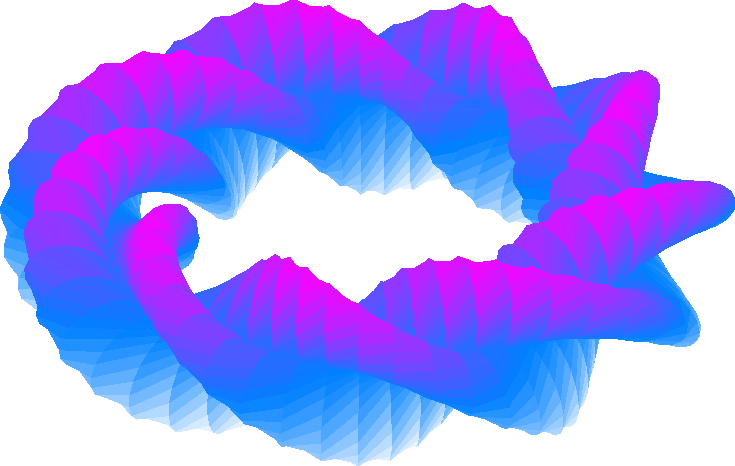
\includegraphics[scale=0.9]{fig/curvy-donut.pdf}
	\end{figure}
	\vspace*{\stretch{2.0}}
	
\end{titlepage}

\tableofcontents

%+-------------------+
%| +---------------+ |
%| |    Chapter    | |
%| +---------------+ |
%+-------------------+
% Topological Spaces


\chapter{Topological Spaces}

%%%%%%%%%%%%%%%%%%%%
% Topological Spaces
%%%%%%%%%%%%%%%%%%%%

\section{Topological Spaces}

{\color{red}Continuous is: points that start "close" end "close"}


\begin{defn}
	Let $X$ be a set, then a \textbf{topology} on $X$ is a collection $\mathcal{T}$ of subsets of $X$ such that
	\begin{enumerate}
		\item $\varnothing, X \in \mathcal{T}$,
		\item $\bigcup_{\alpha\in \mathcal{J}}U_\alpha \in \mathcal{T}$, and
		\item $\bigcap_{i=1}^N U_i \in \mathcal{T}$.
	\end{enumerate}
	Elements of a topology are called \textbf{open sets}.
\end{defn}

\begin{ex}
\begin{enumerate}
	\item ``Indiscrete" topology: $\mathcal{T}_i = \left\{ \varnothing, X \right\}$ 
	\item ``Discrete" topology: $\mathcal{T}_d =\{$all subsets of $X\}$
\end{enumerate}
\end{ex}

\begin{defn}
	Let $\mathcal{T},\mathcal{T}'$ be topologies on a set $X$, then $\mathcal{T}$ is \textbf{finer} than $\mathcal{T}'$ if $\mathcal{T}' \subset \mathcal{T}$. $\mathcal{T}$ is \textbf{coarser} than $\mathcal{T}'$ if $\mathcal{T} \subset \mathcal{T}'$. The notions of \textbf{strictly finer} and \textbf{strictly coarser} follow.
\end{defn}

From this we see that ``fine" is a notion of a large topology, and ``coarse" is a notion of a small topology.

\begin{ex}[]
	The \textbf{lower limit topology} on $\mathbb{R}$ is given by the basis
	\[
		\mathcal{B}= \left\{ [a,b) \;|\; a < b \right\}.
	\] It is strictly finer than the standard topology on $\mathbb{R}$: since $\bigcup_{n\in \mathbb{N}}[a + 1/n, b)=(a,b)$, it contains the standard topology, but $[a,b)$ is not open in the standard topology, so it is strictly finer.
\end{ex}

\begin{ex}[]
	Let $X$ be any set, then the \textbf{finite complement topology} is defined
	\[
		\mathcal{T}_f = \left\{ U \subset X \;|\; X-U \text{ is finite} \right\} \cup\left\{ \varnothing \right\},
	\] 
	where $X-U$ denotes the complement of $U$ in $X$, i.e. $X \backslash U$. Checking that this is a topology boils down to just using DeMorgan's Laws.
\end{ex}

%%%%%%%%%%%%%%%%%%%%
% Bases
%%%%%%%%%%%%%%%%%%%%

\section{Bases}

\begin{defn}
Let $\mathcal{T}$ be a topoloy on $X$, and let $\mathcal{B} \subset \mathcal{T}$. Then $\mathcal{B}$ is a \textbf{basis} for $\mathcal{T}$ if every open set of $\mathcal{T}$ can be written as the union of elements of $\mathcal{B}$.
\end{defn}

\begin{prop}
\label{prop:basis-specific-top}
Let $\mathcal{T}$ be a topology on $X$, and let $\mathcal{B}$ be a collection of subsets of $X$. Then $\mathcal{B}$ is a basis for $\mathcal{T}$ if and only if
\begin{enumerate}
	\item $\mathcal{B}\subset \mathcal{T}$; and
	\item for each $U \in \mathcal{T}$ and $p \in U$, there is a $B \in \mathcal{B}$ such that $p \in B \subset U$.
\end{enumerate}
\end{prop}
\begin{proof}
	The forward direction follows from every open set of $\mathcal{T}$ being the union of elements of $\mathcal{B}$. For the backward direction, since $p \in B_p \subset U$ for all $p \in U$, we have $U = \bigcup_{p\in U}B_p$, so every open set of $\mathcal{T}$ is the union of elements of $\mathcal{B}$. 
\end{proof}

\begin{figure}[H]
	\centering
	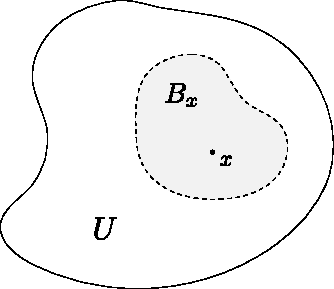
\includegraphics[scale=0.8]{fig/gen-top.pdf}
	\caption{For any $U \in \mathcal{T}$, each $x \in U$ lies in some $B_x \in \mathcal{B}$ for $B_x \subset U$.}
\end{figure}


Not every set of subsets of $X$ will generate a topology, so we need conditions for a collection $\mathcal{B}$ to be a basis for \textit{any} topology.

\begin{prop}
\label{prop:basis-for-any-top}
Let $\mathcal{B}$ be a collection of subsets of $X$. Then $\mathcal{B}$ generates a topology if and only if
\begin{enumerate}
	\item $\bigcup_{B \in \mathcal{B}}=X$.
	\item given $B_1,B_2 \in \mathcal{B}$ and $x \in B_1 \cap B_2$, there is a $B_3 \in \mathcal{B}$ such that $x \in B_3 \subset B_1 \cap B_2$.
\end{enumerate}
\end{prop}
\begin{proof}
	\textbf{Forward:} (1) $X$ must be open, so $X$ is the union of the elements of $\mathcal{B}$. (2) Since $B_1$ and $B_2$ are both open in the topology generated by $\mathcal{B}$, their intersection is, as well. Then since $\mathcal{B}$ is a basis for this topology, we can find a satisfactory $B_3$.

	\textbf{Backward:} The topology generated by a set $\mathcal{B}$ is the collection of all unions of elements of $\mathcal{B}$. It is clear that $\varnothing$ is in it, and condition (1) implies that $X$ is, as well. Arbitrary unions are in the topology by definition. Induction on condition (2) shows that the topology also contains finite intersections.
\end{proof}

\begin{figure}[H]
	\centering
	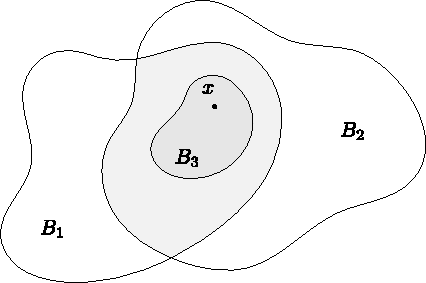
\includegraphics[scale=1]{fig/basis.pdf}
	\caption{Condition $(2)$ in Proposition \ref{prop:basis-for-any-top}.}
\end{figure}

\begin{note}
Since $\mathcal{B}$ exists independently from any topology, it doesn't make sense to describe its members as ``open" until after we've generated a topology from it. Once we've done so, though, it should be clear that every basis element is open in the generated topology.
\end{note}

We can also get a notion of how relatively fine or coarse a topology is by using its basis.

\begin{prop}
	Let $\mathcal{B}, \mathcal{B}'$ be bases for the topologies $\mathcal{T},\mathcal{T}'$ on $X$, respectively. Then $\mathcal{T}'$ is finer than $\mathcal{T}$ if and only if for all $B \in \mathcal{B}$ and $x \in B$, there is a $B' \in \mathcal{B}'$ such that $x \in B' \subset \mathcal{B}$.
\end{prop}
\begin{proof}
	First we show the backward implication. Let $U \in \mathcal{T}$, and let $x \in U$. Since $\mathcal{B}$ generates $\mathcal{T}$, there is a $B \subset \mathcal{B}$ such that $x \in B \subset U$. By assumption, there is then a $B' \in \mathcal{B}'$ such that $x \in B' \subset B \subset U$. Thus $U \in \mathcal{T}'$, so $\mathcal{T}'$ is finer than $\mathcal{T}$.

	Now we show the forward implication. Let $B \in \mathcal{B}$, and let $x \in B$, then $B \in \mathcal{T}$. By assmption, $\mathcal{T} \subset \mathcal{T}'$, so $B \in \mathcal{T}'$ as well. Then by thedefinition of a generated topology, there is a $B' \subset \mathcal{B}'$ such that $x \in B' \subset B$.
\end{proof}

%%%%%%%%%%%%%%%%%%%%
% Subbases
%%%%%%%%%%%%%%%%%%%%

\section{Subbases}

\begin{defn}
	A \textbf{subbasis} $\mathcal{S}$ for a topology $\mathcal{T}$ on $X$ is a collection of subsets of $X$ whose finite intersections form a basis for $\mathcal{T}$.
\end{defn}

Subbases are easier to construct than bases, but the construction of a topology from a subbasis involves an extra step, namely the finite intersections. What we are doing is creating a basis $\mathcal{B}$ from $\mathcal{S}$ by taking finite intersections of the subbasis elements. Then we are taking $\mathcal{B}$ and constructing $\mathcal{T}$ by taking arbitrary unions, as is usual.

\begin{figure}[H]
	\centering
	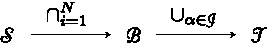
\includegraphics[scale=1]{fig/subbasis-to-topology.pdf}
	\caption{The process for constructing a topology using a subbasis $\mathcal{S}$.}
\end{figure}

{\color{red}Subbasis is smallest set contained in topology or something like that?}

\begin{prop}
Let $\mathcal{T}$ be a topology on $X$, and let $\mathcal{S}$ be a collection of subsets of $X$. Then $\mathcal{S}$ is a subbasis for $\mathcal{T}$ if and only if
\begin{enumerate}
	\item $\mathcal{S} \subset \mathcal{T}$; and
	\item for each $U \in \mathcal{T}$ and $p \in U$, there is a finite intersection $\bigcap_{i=1}^n S_i$ of elements of $\mathcal{S}$ such that $p \in \bigcap_{i=1}^n S_i \subset U$.
\end{enumerate}
\end{prop}
\begin{proof}
	This follows from Proposition \ref{prop:basis-specific-top} (the analogue of this proposition for bases). When proving both directions, there's just an extra step to go from a genric basis element to a finite intersection of elements of $\mathcal{S}$.
\end{proof}

Just as with bases, we have a condition for when an arbitrary collection of subsets of $X$ can be a valid subbasis.

\begin{prop}
Let $\mathcal{S}$ be a collection of subsets of $X$. Then $\mathcal{S}$ generates a topology if and only if every point of $X$ is in some element of $\mathcal{S}$.
\end{prop}
\begin{proof}
{\color{red}Sketch.}
\end{proof}

%%%%%%%%%%%%%%%%%%%%
% The Subspace Topology
%%%%%%%%%%%%%%%%%%%%

\section{The Subspace Topology}

There is a natural way of a subset inheriting the topology of the set it lies in. The following definition is easily checked to actually be a topology.

\begin{defn}
	Let $(X,\mathcal{T})$ be a topological space. If $Y \subset X$, then
	\[
	\mathcal{T}_Y = \left\{ Y \cap U \;|\; U \in \mathcal{T} \right\}
	\] is the \textbf{subspace topology} on $Y$. With this topology, $Y$ is called a \textbf{subspace} of $X$.
\end{defn}

\begin{prop}
Let $\mathcal{B}$ be a basis for the topology of $X$, then \[\mathcal{B}_Y \doteq \left\{ B \cap Y \;|\; B \in \mathcal{B} \right\}\] is a basis for the subspace topology on $Y$.
\end{prop}
\begin{proof}
	Let $y \in U \cap Y$, where $U$ is open in $X$. There exists $B \in \mathcal{B}$ such that $y \in B \subset U$, so $y \in B \cap Y \subset U \cap Y$.
\end{proof}

\begin{prop}
	Let $Y$ be a subspace of $X$, and let $U$ be open in $Y$ and $Y$ be open in $X$. Then $U$ is open in $X$.
\end{prop}
\begin{proof}
	$U$ is open in $Y$, so $U=Y \cap V$ for some $V$ open in $X$. Both sets $Y$ and $V$ are open in $X$, so their intersection $U$ must be as well.
\end{proof}

%%%%%%%%%%%%%%%%%%%%
% The Product Topology
%%%%%%%%%%%%%%%%%%%%

\section{The Product Topology}

It would be natural to define the product topology as
\[
	\mathcal{P}= \left\{ U \times V \;|\; U \text{ open in } X, V \text{ open in } Y \right\},
\]but this isn't enough to give a topology since you can construct examples where the union of elements in this set don't lie in the set.

This set \textit{is}, however, perfectly valid as a basis, since $\bigcup_{U,V}(U\times V)=X\times Y$ and $(U_1 \times V_1) \cap (U_2 \times V_2) = (U_1 \cap U_2) \times (V_1 \cap V_2) \in \mathcal{P}$.

\begin{defn}[]
The topology generated by $\mathcal{P}$ is the \textbf{product topology} on $X \times Y$.
\end{defn}

\begin{prop}
If $\mathcal{B}_X$ is a basis for $X$ and $\mathcal{B}_Y$ is a basis for $Y$, then $\mathcal{B}_X \times \mathcal{B}_Y$ is a basis for the product topology.
\end{prop}

\begin{prop}
	The product and subspace topologies ``commute".
\end{prop}
\begin{proof}
	It's straightforward to show that the product of two subspaces and the subspace of a product both have the same basis.
\end{proof}


%%%%%%%%%%%%%%%%%%%%
% Closed Sets and Limit Points
%%%%%%%%%%%%%%%%%%%%

\section{Closed Sets and Limit Points}

\begin{defn}
	A set $A \subset (X, \mathcal{T})$ is closed if $X-A$ is open in $X$.
\end{defn}

\begin{thrm}
	Let $(X, \mathcal{T})$ be a topological space, and let $F$ denote a closed set of $X$, then
	\begin{enumerate}
		\item $\varnothing$ and $X$ are closed,
		\item $\bigcap_{\alpha\in\mathcal{J}}F_\alpha$ is closed, and
		\item $\bigcup_{i=1}^N F_i$ is closed.
	\end{enumerate}
\end{thrm}
\begin{proof}
This is a straightforward application of DeMorgan's Laws.
\end{proof}

\begin{prop}
	\label{closed-isct}
Let $Y$ be a subspace of $X$. Then $A$ is closed in $Y$ if and only if it is equal to the intersection of a closed set of $X$ with $Y$.
\end{prop}
\begin{proof}
	First we show the forward implication. Assume $A$ is closed in $Y$, then $Y-A$ is open in $Y$, so be definition $Y-A=U \cap Y$ for some $U$ open in $X$. $X-U$ is closed in $X$, and $A = Y \cap (X-U)$, so $A$ is the intersection of a closed set of $X$ with $Y$.

	Now we show the backward implication. Assume $A = C \cap Y$ for $C$ closed in $X$. Then $X-C$ is open in $X$, so $(X-C) \cap Y$ is open in $Y$ by the definition of the subspace topology. But $(X-C) \cap Y = Y-A$, so $Y-A$ is open in $Y$. Thus $A$ is closed in $Y$.
\end{proof}

\begin{prop}
Let $Y$ be a subspace of $X$. If $A$ is closed in $Y$ and $Y$ is closed in $X$, then $A$ is closed in $X$.
\end{prop}
\begin{proof}
	$A = F \cap Y$ for some $F$ closed in $X$. $A$ is then the intersection of closed sets of $X$, so it is itself closed in $X$.
\end{proof}

\begin{defn}
	The \textbf{interior} of a set $A$, denoted $A^o$, is the union of all open sets contained in $A$.

	The \textbf{closure} of a set $A$, denoted $\overline{A}$ is the intersection of all closed sets containing $A$.
\end{defn}

The closure of a set is clearly closed, and the interior of a set is clearly open. It is also clear that if $A$ is open, then $A^o = A$, and if $A$ is closed, then $\overline{A}=A$. We also have the obvious relation $A^o \subset A \subset \overline{A}$.

We have to be careful when describing closures. Given a subspace $Y$ of $X$, the closure of $A$ in $X$ is generally not the same as the closure of $A$ in $Y$. In this case, we use $\overline{A}$ to denote the closure of $A$ in $X$ (the overall space). We relate this to the closure of $A$ in $Y$ (the subspace) with the following proposition.

\begin{prop}
	Let $Y$ be a subspace of $X$, and let $A \subset Y$. Denote the closure of $A$ in $X$ by $\overline{A}$. Then the closure of $A$ in $Y$ is equal to $\overline{A} \cap Y$.
\end{prop}
\begin{proof}
	Let $B$ denote the closure of $A$ in $Y$. $\overline{A}$ is closed in $X$, so by Proposition \ref{closed-isct}, $\overline{A} \cap Y$ is closed in $Y$. Since $\overline{A} \cap Y$ contains $A$, and since by definition $B$ is the intersection of all closed subsets of $Y$ containing $A$, we have $B \subset \overline{A}\cap Y$.

	On the other hand, we know $B$ is closed in $Y$. Again by Proposition \ref{closed-isct}, $B = C \cap Y$ for some $C$ closed in $X$. Then $C$ is a closed set of $X$ containing $A$. Since $\overline{A}$ is the intersection of all such closed sets, we have $\overline{A} \subset C$, so $(\overline{A} \cap Y) \subset (C \cap Y) = B$.
\end{proof}

\begin{defn}
A \textbf{neighborhood} of a point $X$ is an open set containing $x$.
\end{defn}

\begin{thrm}
	\label{thrm:nhood-closure}
Let $A$ be a subset of a topological space $X$, then
\begin{enumerate}
	\item $x \in \overline{A}$ if and only if every neighborhood of $x$ intersects $A$, and
	\item Supposing the topology of $X$ is given by a basis, then $x \in \overline{A}$ if and only if every basis element $B$ containing $x$ intersects $A$.
\end{enumerate}
\end{thrm}
\begin{proof}
	\begin{enumerate}
		\item We'll prove the contrapositive: $x \not\in \overline{A}$ if and only if there exists an open neighborhood of $x$ that does not intersect $A$. We will first show the forward implication. Assume $x \not\in \overline{A}$, then $U = X-\overline{A}$ is open, contains $x$, and does not intersect $A$.

			Now we show the backward implication. Assume there exists an open neighborhood $U$ of $x$ that does not intersect $A$, then $X-U$ is a closed set containing $A$. By the definition of $\overline{A}$, $X-U$ must contain $\overline{A}$. Thus $x \not\in \overline{A}$.

		\item First we show the forward implication. By (1) we know if $x \in  \overline{A}$, then every open neighborhood of $x$ intersects $A$. Since basis elements are open, this implies that every basis element containing $x$ intersects $A$.

			Now we show the backward implication. Assume every basis element containing $x$ intersects $A$. Since every open neighborhood $U$ of $x$ contains some basis element, every such $U$ also intersects $A$. Again by (1), this implies $x \in \overline{A}$.
	\end{enumerate}
\end{proof}

\begin{defn}
	Let $A \subset (X,\mathcal{T})$, then $x \in X$ is a \textbf{limit point}/cluster point/accumulation point of $A$ if every open neighborhood of $x$ intersects $A$ at some point \textit{other than $x$ }.

	Equivalently, $x$ belongs to the closure of $A - \left\{ x \right\}$. Note that $x$ need not lie in $A$.
\end{defn}

\begin{thrm}
	Let $A \subset (X,\mathcal{T})$, and denote the set of limit points of $A$ by $A'$. Then $\overline{A}=A \cup A'$.
\end{thrm}
\begin{proof}
	First we show $A' \cup A \subset \overline{A} $. Let $x \in A'$, then every open neighborhood of $x$ intersects $A$ (at a point other than $x$). Thus by Theorem \ref{thrm:nhood-closure}, $x \in \overline{A}$, so $A' \subset  \overline{A}$. Since $A \subset \overline{A}$ by definition, we have $A \subset A' \subset \overline{A}$.

	Now we show $\overline{A} \subset A' \cup A$. Let $x \in \overline{A}$. If $x \in A$, then this is trivial, so assume $x \not\in A$. Since $x \in \overline{A}$, every neighborhood of $x$ intersects $A$. Since $x \not\in A$, this must be at a point other than $x$. Thus $x \in A'\subset A' \cup A$, so $\overline{A} \subset A' \cup A$.
\end{proof}

\begin{cor}
	A subset of a topological space is closed if and only if it contains all its limit points.
\end{cor}
\begin{proof}
	Let $A \subset (X, \mathcal{T})$. Then $A$ is closed if and only if $A = \overline{A} = A \cup A'$, and $A = A \cup A'$ if and only if $A' \subset A$.
\end{proof}


%+-------------------+
%| +---------------+ |
%| |    Chapter    | |
%| +---------------+ |
%+-------------------+
% Separation Properties

\chapter{Separation Properties}

%%%%%%%%%%%%%%%%%%%%
% Convergence
%%%%%%%%%%%%%%%%%%%%

\section{Convergence}

We say that a sequence $\left\{ x_n \right\}$ is \textbf{eventually} in $U$ if there is some $N$ such that $x_n \in U$ when $n \geq N$.

\begin{defn}[]
$\left\{ x_n \right\}$ \textbf{converges} to $x$ if it's eventually in every open neighborhood of $x$.
\end{defn}

\begin{ex}[]
In the discrete topology, $x_n \to x$ if $\left\{ x_n \right\}$ eventually equals $x$.

In the indiscrete topology, every sequence converges to every point.
\end{ex}
If we want limits to be unique, we have to enforce certain separation axioms.


%%%%%%%%%%%%%%%%%%%%
% The Separation Axioms
%%%%%%%%%%%%%%%%%%%%

\section{The Separation Axioms}

Turns out that separating points yields some nice properties of topological spaces. Who'da thunk?

{\color{red}Stuff about $T_1$-$T_4$. Theorems about how they're related.}

\begin{figure}[H]
	\centering
	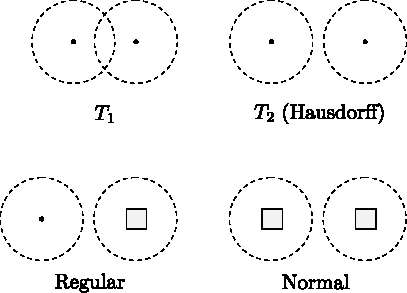
\includegraphics[scale=1]{fig/separation.pdf}
	\caption{The four main types of separation.}
\end{figure}

\begin{prop}
	Let $X$ be $T_1$, and let $A$ be a subset of $X$. Then $x$ is a limit point of $A$ if and only if every neighborhood of $x$ contains infinitely many points of $A$.
\end{prop}
\begin{proof}
	\textbf{Backward:} Every neighborhood of $x$ intersects $A$ at infinitely many points, so it they surely all intersect $A$ at a point other than $x$. Thus $x$ is a limit point.

	\textbf{Forward:} Let $x$ be a limit point of $A$, and suppose some neighborhood $U$ of $x$ intersects $A$ at only finitely many points. Let $\left\{ x_1,\dots,x_m \right\} = U \cap (A-\left\{ x \right\})$, then $X - \left\{ x_1,\dots,x_m \right\}$ is open in $X$ since $X$ satisfies the $T_1$ axiom. Then $U \cap (X - \left\{ x_1,\dots,x_m \right\})$ is a neighborhood of $x$ that doesn't intersect $A - \left\{ x \right\}$ at all. This contradicts $x$ being a limit point of $A$, so every neighborhood of $x$ must intersect $A$ at infinitely many points.
\end{proof}

\begin{prop}
	A space is $T_1$ if and only if all single points are closed.
\end{prop}
\begin{proof}
	\textbf{Forward:} Suppose $X$ is $T_1$, then fix $x \in X$. Then for $y \in X- \left\{ x \right\}$, there is an open $U_{y}$ such that $y \in U_y \subset X - \left\{ x \right\}$, so $X - \left\{ x \right\} = \bigcup_{y}U_y$. Then $X-\left\{ x \right\}$ is open so $\left\{ x \right\}$ is closed.

	\textbf{Backward:} Suppose all single points in $X$ are closed. Fix $x,y \in X$, then $X-\left\{ x \right\}$ and $X-\left\{ y \right\}$ are the open sets we need to show that $X$ is $T_1$.
\end{proof}

\begin{cor}
	A space is $T_1$ if and only if all finite point sets are closed.
\end{cor}
\begin{proof}
	{\color{red}Do I even need one? Kinda obvious.}
\end{proof}

%%%%%%%%%%%%%%%%%%%%
% Hausdorff Spaces
%%%%%%%%%%%%%%%%%%%%

\section{Hausdorff Spaces}

\begin{prop}
	Every finite set in a Hausdorff space is closed.
\end{prop}
\begin{proof}
	Hausdorff spaces are $T_1$.
\end{proof}

\begin{prop}
	Let $X$ be a Hausdorff space, then a sequence of points in $X$ converges to at most one point in $X$.
\end{prop}
\begin{proof}
	Suppose $\left\{ x_n \right\} \subset X$ such that $x_n \to x \in X$. If $y \neq x$, then since $X$ is Hausdorff we can find disjoint open neighborhoods $U$ and $V$of $x$ and $y$, respectively. The set $U$ contains all but finitely many of the points in $\left\{ x_n \right\}$, so $V$ can only contain finitely many of the points in $\left\{ x_n \right\}$. Thus $x_n$ cannot converge to $y$.
\end{proof}

\begin{prop}
	Every simply ordered set is Hausdorff in the order topology.
\end{prop}
\begin{proof}
	{\color{red}Do this.}
\end{proof}

\begin{prop}
	The product of two Hausdorff spaces is a Hausdorff space.
\end{prop}
\begin{proof}
	{\color{red}Do this.}
\end{proof}

\begin{prop}
	A subspace of a Hausdorff space is Hausdorff.
\end{prop}
\begin{proof}
	Suppose $X$ is Hausdorff and that $Y$ is a subspace of $X$ with distinct points $u$ and $v$. Then $u$ and $v$ are also distinct points of $X$, so by the regularity of $X$, they are separated by disjoint open sets $U$ and $V$ in $X$. Then $Y \cap U$ and $Y \cap V$ are the desired open sets of $Y$.
\end{proof}

%%%%%%%%%%%%%%%%%%%%
% Regular Spaces
%%%%%%%%%%%%%%%%%%%%

\section{Regular Spaces}

\begin{prop}
$X$ is regular if and only if for all $p \in X$ and open neighorhood $U$ of $p$, there is an open set $V$ such that $p \in V$ and $\overline{V}\subset U$.
\end{prop}
\begin{proof}
	{\color{red}Do this. Forward direction already in written notes so don't throw out that paper yet.}
\end{proof}

\begin{prop}
Every subspace of a regular space is regular.
\end{prop}
\begin{proof}
	Let $Y$ be a subspace of a regular space $X$, let $A$ be closed in $Y$, and let $y \in Y-A$. Then $A = \text{cl}_X(A) \cap Y$, and $\text{cl}_X(A)$ is a closed set in $X$ not containing $y$. Then the regularity of $Y$ follows from the regularity of $X$.
\end{proof}

%%%%%%%%%%%%%%%%%%%%
% Normal Spaces
%%%%%%%%%%%%%%%%%%%%

\section{Normal Spaces}

\begin{prop}
	\label{prop:normal-iff}
	$X$ is normal if and only if for all closed sets $A$ and open sets $U$ containing $U$, there exists an open set $V$ such that $A \subset V$ and $\overline{V}\subset U$.
\end{prop}
\begin{proof}
{\color{red}Hey there.}
\end{proof}

\begin{prop}
$X$ is normal if and only if for all pairs of disjoint closed sets $A$ and $B$, there are disjoint open containing $A$ and $B$ whose closures are also disjoint.
\end{prop}
\begin{proof}
{\color{red}These really be piling up.}
\end{proof}

Suppose a space is normal and covered by 2 open sets. Then we can actually find two smaller patches (smaller in the sense that their closures are contained in the original patches) that cover the space too.

\begin{thrm}[The Shrinking Theorem]
$X$ is a normal topological space if and only if for all open covers $\left\{ U,V \right\}$ of $X$, there exist open sets $U'$ and $V'$ such that $\overline{U'} \subset U$, $\overline{V'} \subset V$, and $U'$ and $V'$ also cover $X$.
\end{thrm}
\begin{proof}
	\textbf{Forward:} Suppose $X$ is normal and is covered by open sets $U$ and $V$. Note that $X-U$ is closed and is a subset of $V$. Then by Proposition \ref{prop:normal-iff}, there exists an open set $V'$ such that $X-U \subset V' \subset \overline{V'} \subset V.$

	Then $U \cup V'$ contains $U \cup X-U = X$, so $\left\{ U,V' \right\}$ is an open cover of $X$. We can repeat this argument to replace $U$ with the desired $U'$.

	\textbf{Backward:} Let $A$ be closed in $X$ and contained in some open set $U$ of $X$. Again by Proposition \ref{prop:normal-iff}, we need to find an open set $U'$ such that $A \subset U'$ and $\overline{U'} \subset U$.

	Since $X-A$ is open and $X-A$ and $U$ cover $X$, by assumption, there exist open $U'$ and $V'$ such that $\overline{U'} \subset U$, $\overline{V'} \subset X-A$, and $U' \cup V' = X$. We claim that $U'$ is our desired open set. We already have $\overline{U'}  \subset U$, so we only need to show $A \subset U'$.

	Now $U'$ and $V'$ cover $X$, so $X-V' \subset U'$. Additionally, $V' \subset X-A$. Together, these give $A \subset X-V' \subset U'$.
\end{proof}

{\color{red}Extenstion of this theorem to more than 2 open sets.}

A somewhat surprising result is that not all subspaces of normal spaces are normal. To see why, we can modify the earlier proof that subspaces of regular spaces are themselves regular. Let $Y$ be a subspace of a normal space $X$, and let $A$ and $B$ be closed in $Y$. Then
\[
	A= \text{cl}_X(A) \cap Y, B = \text{cl}_X(B) \cap Y.
\] In order to use the regularity of $X$, we would need $\text{cl}_X(A)$ and $\text{cl}_X(B)$ to be disjoint. Unfortunately, this is not true in general (see the figure below). It \textit{is} true, though, if $Y$ is a closed subspace of $X$.

\begin{figure}[H]
	\centering
	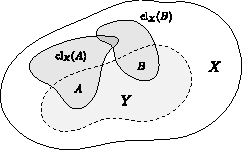
\includegraphics[scale=2]{fig/normal-counter.pdf}
	\caption{An exaggerated example of what could happen if $Y$ is open in $X$.}
\end{figure}


\begin{prop}
Closed subspaces of normal spaces are normal.
\end{prop}
\begin{proof}
	Let $Y$ be a closed subspace of a normal space $X$, and let $A$ and $B$ be closed in $Y$. Then since $Y$ is closed in $X$, both $A$ and $B$ are also closed in $X$. Then the normality of $Y$ follows from the normality of $X$.
\end{proof}

\begin{defn}
$A,B \subset X$ are \textbf{separated} if $\overline{A}\cap B$ and $A \cap \overline{B}$ are both empty, i.e. they don't contain each other's limit points.
\end{defn}

{\color{red}I need a line break here.}

\begin{defn}
$X$ is \textbf{completely normal} if for any two separated sets $A$ and $B$, there exist disjoint open sets $U$ and $V$ such that $A \subset U$ and $B \subset V$. A $T_5$ space is any space that is both $T_1$ and completely normal.
\end{defn}

\begin{lem}
	Let $Y$ be a subspace of $X$, and let $A$ and $B$ be disjoint closed sets in $Y$. Then $A$ and $B$ are separated in $X$.
\end{lem}
\begin{proof}
	Denote the closure in $X$ with a bar, then $A=\overline{A} \cap Y$ and $B = \overline{B}\cap Y$. Then $\overline{A} \cap B = A \cap \overline{B}= \overline{A}\cap \overline{B}\cap Y = A \cap B = \varnothing$.
\end{proof}

\begin{prop}
$X$ is completely normal if and only if every subspace of $X$ is normal.
\end{prop}
\begin{proof}
\textbf{Forward:} Let $A$ and $B$ be closed in a subspace $Y$ of $X$, then by the previous lemma, they are separated in $X$. Since $X$ is completely normal, there are disjoint open sets $U$ and $V$ of $X$ such that $A \subset U$ and $B \subset V$. Then $U \cap Y$ and $V\cap Y$ are the desired open sets to show that the subspace $Y$ is normal.

\textbf{Backward:} Let $A$ and $B$ be separated in $X$, then $A \in X- \overline{B}$ and $B \in X-\overline{A}$. Consider the subspace $Y \doteq (X-\overline{B}) \cup (X-\overline{A}) = X - (\overline{B} \cap \overline{A})$. Then since $\text{cl}_Y(A) = \overline{A}\cap Y$ and $\text{cl}_y(B) = \overline{B}\cap Y$, the definition of $Y$ gives $\text{cl}_Y(A) \cap \text{cl}_Y(B) = \overline{A} \cap \overline{B} \cap Y = \varnothing$.

Then since $\text{cl}_Y(A)$ and $\text{cl}_Y(B)$ are disjoint and closed in $Y$, and since $Y$ is normal by assumption, there are disjoint open sets $U$ and $V$ of $Y$ such that $\text{cl}_Y(A) \subset U$ and $\text{cl}_Y(B) \subset V$. Then $A \subset U$ and $B \subset V$, so $X$ is completely normal.
\end{proof}


%+-------------------+
%| +---------------+ |
%| |    Chapter    | |
%| +---------------+ |
%+-------------------+
% Continuity

\chapter{Continuity}

%%%%%%%%%%%%%%%%%%%%
% Continuous Functions
%%%%%%%%%%%%%%%%%%%%

\section{Continuous Functions}

In the category of topological spaces, the morphisms are continuous functions.

\begin{defn}
	Let $X,Y$ be topological spaces, then $f : X \to Y$ is \textbf{continuous} if for all $U$ open in $Y$, $f^{-1}(U)$ is open in $X$.
\end{defn}

\begin{prop}
	If $Y$ has basis $\mathcal{B}$ and $f^{-1}(B)$ is open in $X$ for all $B \in \mathcal{B}$, then $f: X \to Y$ is continuous.
	Similarly, if $Y$ has subbasis $\mathcal{S}$ and $f^{-1}(S)$ is open in $X$ for all $S \in \mathcal{S}$, then $f: X \to Y$ is continuous.
\end{prop}
\begin{proof}
	The preimage of any open set if the union of preimages of basis elements. The preimage of any basis element is the finite intersection of preimages of subbasis elements.
\end{proof}

\begin{thrm}
Let $X$ and $Y$ be topological spaces, and let $f: X \to Y$, then the following are equivalent:
\begin{enumerate}
	\item $f$ is continuous.
	\item For all $A \subset X$, $f(\overline{A}) \subset \overline{f(A)} $.
	\item For all $B$ closed in $Y$, $f^{-1}(B)$ is closed in $X$.
	\item For all $x \in X$ and for each neighborhood $V$ of $f(x)$, there is a neighborhood $U$ of $x$ such that $f(U) \subset V$.
\end{enumerate}
\end{thrm}

As with any category, the isomorphisms of \textbf{Top} are invertible morphisms.

\begin{defn}
	Let $X$ and $Y$ be topological spaces, and let $f: X \leftrightarrow Y$ be bijective. If $f$ and $f^{-1}$ are continuous, then $f$ is a \textbf{homeomorphism}.

	Equivalently, a homeomorphism is a bijective function $f: X \leftrightarrow Y$ such that $U$ is open in $X$ if and only if $f(U)$ is open in $Y$.
\end{defn}

\begin{figure}[H]
	\centering
	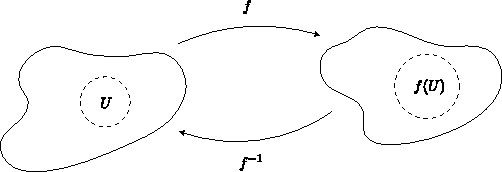
\includegraphics[scale=1.3]{fig/homeomorphism.pdf}
	\caption{A homeomorphism $f$.}
\end{figure}

\begin{defn}
	A \textbf{topological property} is a property of topological space $X$ expressed entirely in terms of the topology on $X$ (the open sets of $X$).
\end{defn}

If $f:X \to Y$ is a homeomorphism, then $Y$ has the topological properties of $X$.

\begin{defn}
	Suppose $f: X \to  Y$ is one-to-one and continuous. Then $f':X \to  f(X)$ (obtained by restricting the range of $f$) is bijective. If $f'$ is a homeomorphism of $X$ with $f(X)$, we say $f: X \hookrightarrow  Y$ is a \textbf{(topological) embedding} of $X$ in $Y$.
\end{defn}

\begin{thrm}[The Pasting Lemma]
	Let $X = A \cup B$, where $A$ and $B$ are either both closed or both open in $X$. Let $f:A \to Y$ and $g:B\to Y$ be continuous. If $f(x)=g(x)$ for all $x \in A \cap B$, then the function $h : X \to Y$ given by
	\[
		H(x)=
		\begin{cases}
			f(x) & x \in A \\
			g(x) & x\in B
		\end{cases}
	\] is continuous.
\end{thrm}
\begin{proof}
	Suppose $A$ and $B$ are both closed. Let $C$ be closed in $Y$, then $h^{-1}(C) = f^{-1}(C) \cup g^{-1}(C)$. Since $f$ and $g$ are continuous, both $f^{-1}(C)$ and $g^{-1}(C)$ are closed in $A$ and $B$, respectively. Since both $A$ and $B$ are closed in $X$, both preimages are also closed in $X$. Thus $h^{-1}(C)$ is closed and $h$ is subsequently continuous.

	To show this when $A$ and $B$ are both open, replace the word ``closed" with the word ``open" in the above paragraph.
\end{proof}

	Note that the condition $f(x) = g(x)$ for all $x \in A \cap B$ is not needed in this proof. It is only necessary to make $h$ an actual function.

\begin{thrm}[Maps into Products]
	Define $f:A\to X \times Y$ by $f(a)=(f_1(a), f_2(a))$, for $f_1:A\to X$ and $f_2:A\to Y$. Then $f$ is continuous if and only if $f_1$ and $f_2$ are both continuous.
\end{thrm}
\begin{proof}
	Let $\pi_1:X\times Y\to X$ and $\pi_2:X\times Y\to Y$ be the obvious projections, which we know to be continuous.

	We begin with the forward implication. Suppose $f$ is continuous, then $f_1=\pi_1 \circ f$ and $f_2=\pi_2 \circ f$, so $f_1$ and $f_2$ are compositions of continuous functions. Thus they are both continuous themselves.

	Now we show the backward implication. Suppose $f_1$ and $f_2$ are continuous, then we'll show that for each basis element $U \times V$ of the topology on $X \times Y$, the preimage $f^{-1}(U \times V)$ is open. Take a point in the preimage $a \in f^{-1}(U \times V)$, then $f(a) \in U \times V$, so $f_1(a) \in U$ and $f_2(a) \in V$. Thus we have
	\[
		f^{-1}(U \times V) = f_1^{-1}(U) \cap f_2^{-1}(V).
	\] Since $U$ and $V$ are open and $f_1$ and $f_2$ are continuous, both of the sets in the above intersection are open. The finite intersection of open sets is open, so $f^{-1}(U\times V)$ is open, so $f$ is continuous.
\end{proof}

\begin{note}
	If $f:A\times B\to X$ instead, there is \textit{no} useful criterion for the continuity of $f$.
\end{note}

%%%%%%%%%%%%%%%%%%%%
% Constructing Continuous Functions
%%%%%%%%%%%%%%%%%%%%

\section{Constructing Continuous Functions}

\begin{prop}
Constant functions are continuous.
\end{prop}
\begin{proof}
	Let $f:X\to Y$ be given by $f(x)=y$ for some constant $y$. If $V$ is open in $Y$, then $f^{-1}(V)$ is either $\varnothing$ or $X$, depending on if $y \in V$. In either case, $f^{-1}(V)$ is open.
\end{proof}

\begin{prop}
Inclusion maps are continuous.
\end{prop}
\begin{proof}
	Let $X \subset Y$, and define $\iota:X\to Y$ by $\iota(x)=x$. For $V$ open in $Y$, $\iota^{-1}(V)=X \cap V$, which is open in $X$ by definition.
\end{proof}

\begin{prop}
Restrictions of continuous maps are continuous.
\end{prop}
\begin{proof}
	Let $f:X\to Y$ be continuous, and let $A \subset X$. Define $f|_{A}:A\to Y$ by $f|_{A}(a)=f(a)$. For $V$ open in $Y$, $f|_{A}^{-1}(V) = f^{-1}(V) \cap A$, which is open in $A$ since $f^{-1}(V)$ is open in $X$.
\end{proof}

\begin{prop}
Compositions of continuous functions are continuous.
\end{prop}
\begin{proof}
	Let $f:X\to Y$ and $g:Y\to Z$ be continuous. For $V$ open in $Z$, $(g \circ f)^{-1}(V) = f^{-1}(g^{-1}(V))$, which is open in $X$ since $f$ and $g$ are both continuous.
\end{proof}


\end{document}
